\documentclass[letterpaper]{article} % Feel free to change this
\usepackage{graphicx}
\graphicspath{{images/}}

\begin{document}

\title{ECE 350: Digital Systems Homework 6}
\author{Aman Ibrahim} % Change this to your name
\date{\today} % Change this to the date you are submitting
\maketitle

\section*{Duke Community Standard}

By submitting this \LaTeX{} document, I affirm that
\begin{enumerate}
    \item I understand that each \texttt{git} commit I create in this repository is a submission.
    \item I affirm that each submission complies with the Duke Community Standard and the guidelines set forth for this assignment.
    \item I further acknowledge that any content not included in this commit under the version control system cannot be considered as a part of my submission.
    \item Finally, I understand that a submission is considered submitted when it has been received by the server.
\end{enumerate}

\newpage

\section{Answers}

\begin{enumerate}
  \item Decreasing frequency: \\
    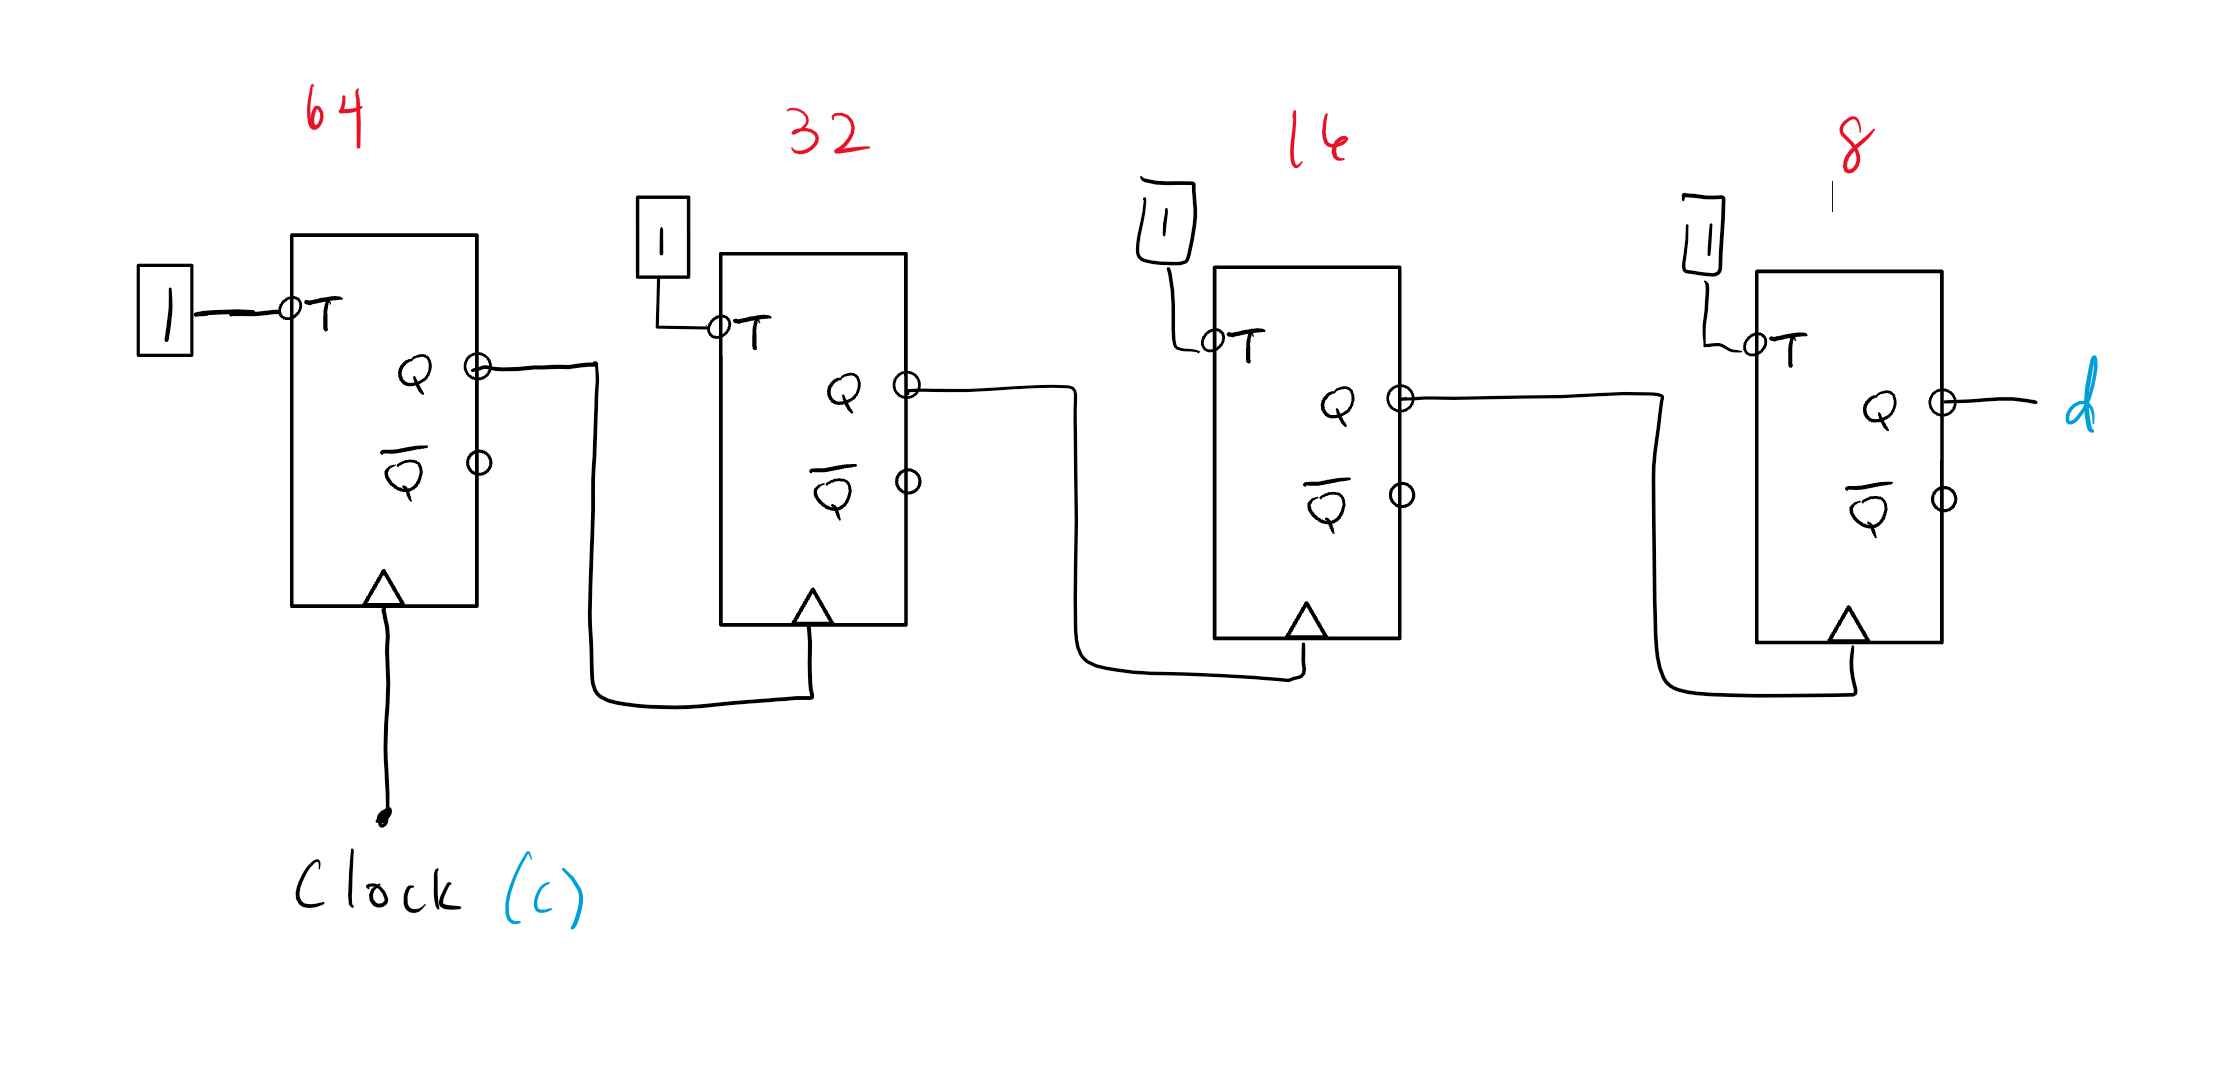
\includegraphics[scale=0.4]{q1}
  \item
  \begin{enumerate}
    \item D Flipflop: \\ \\

    Table: \\ \\
    \begin{tabular}{| lll | lll |}
    \hline
    \multicolumn{3}{| l |}{prev State} & \multicolumn{3}{| l |}{next State} \\
    in0      & in1      & in2      & out0     & out1     & out2     \\
    \hline
    1        & 0        & 0        & 0        & 0        & 0        \\
    0        & 0        & 0        & 0        & 0        & 1        \\
    0        & 0        & 1        & 0        & 1        & 1        \\
    0        & 1        & 1        & 1        & 1        & 1        \\
    1        & 1        & 1        & 1        & 1        & 0        \\
    1        & 1        & 0        & 1        & 0        & 0  \\ \hline
    \end{tabular} \\ \\
    Boolean Expressions: \\
    $out0$ = in1 \\
    $out1$ = in2 \\
    $out3$ = !in0 \\ \\

    Circuit: \\ \\
     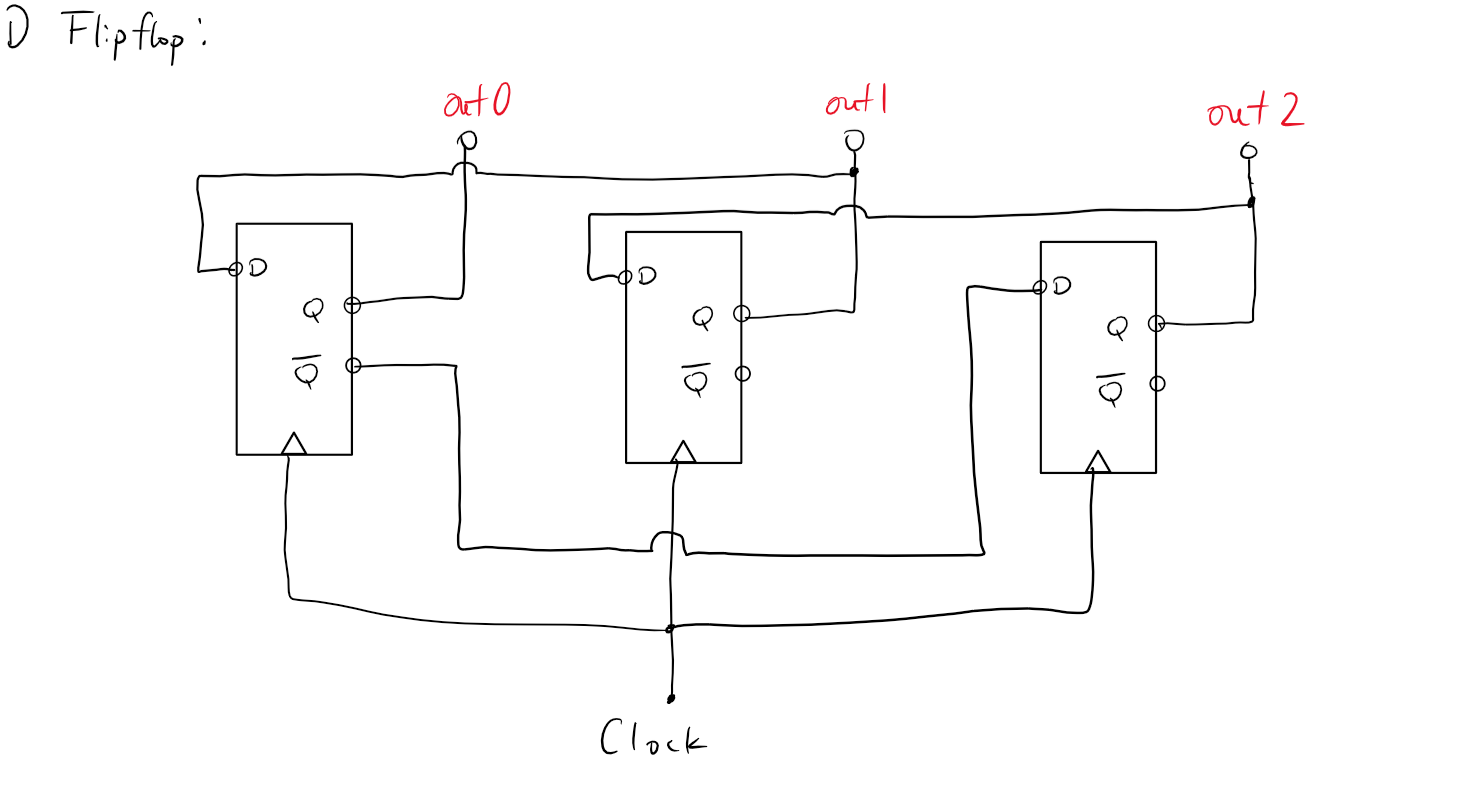
\includegraphics[scale=0.4]{dffe}
    \item T Flipflop: \\ \\

    Table: \\ \\
    \begin{tabular}{|lll|lll|}
      \hline
      \multicolumn{3}{|l|}{prev State} & \multicolumn{3}{|l|}{toggle} \\
      \hline
      in0      & in1      & in2      & t0      & t1      & t2     \\
      \hline
      0        & 0        & 0        & 0       & 0       & 1      \\
      0        & 0        & 1        & 0       & 1       & 0      \\
      0        & 1        & 1        & 1       & 0       & 0      \\
      1        & 1        & 1        & 0       & 0       & 1      \\
      1        & 1        & 0        & 0       & 1       & 0      \\
      1        & 0        & 0        & 1       & 0       & 0  \\
      \hline
    \end{tabular} \\ \\

    Boolean Expressions: \\
    $t0$ = !in1*in2*in3 + in1*!in2*!in3 \\
    $t1$ = !in1*!in2*in3 + in1*in2*!in3 \\
    $t2$ = !in1*!in2*!in3 + in1*in2*in3 \\ \\

    Circuit: \\ \\
    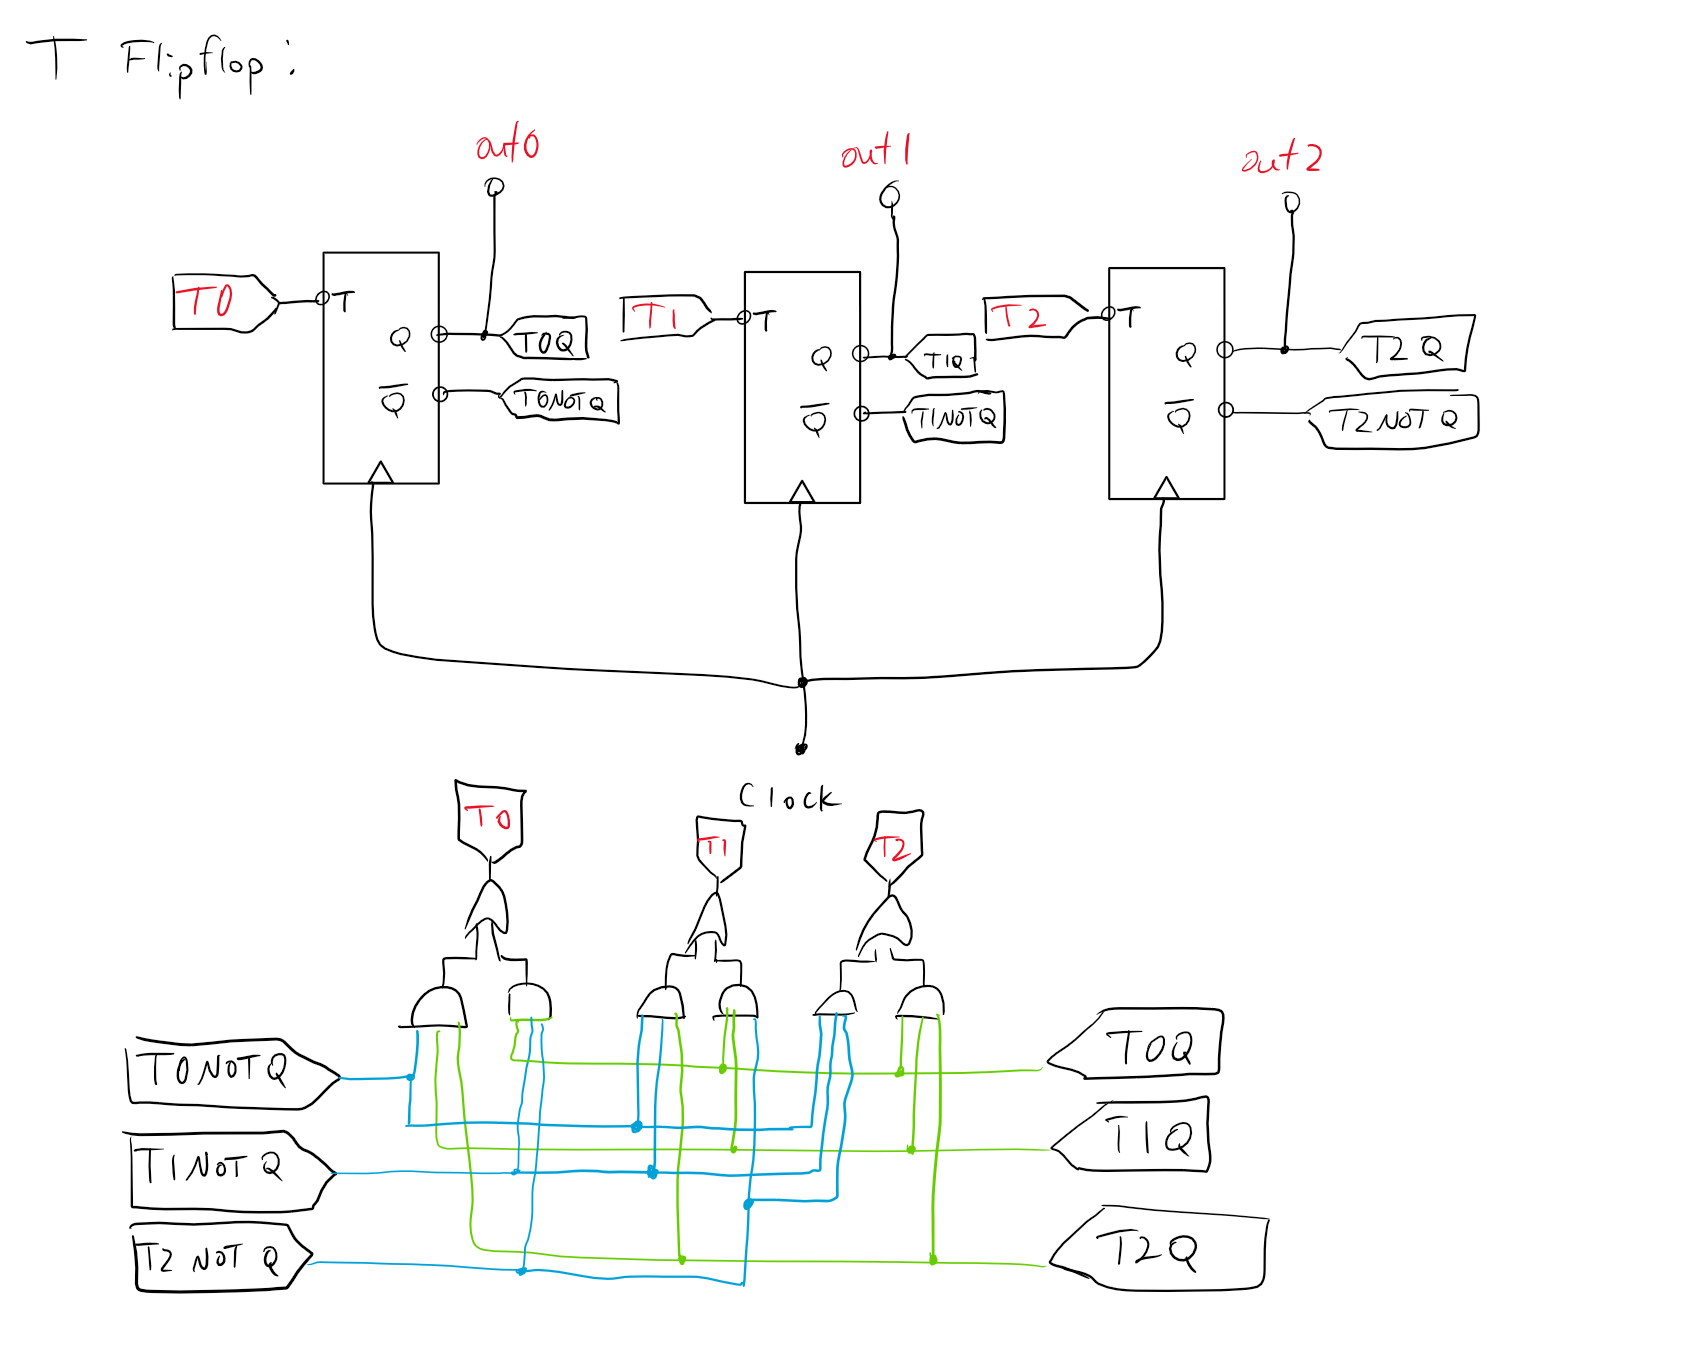
\includegraphics[scale=0.4]{tff}

    \item JK Flipflop: \\ \\
      JK Table: \\ \\
      \begin{tabular}{|l|l|}
        \hline
        JK & Q(t+1)          \\
        \hline
        00 & Q(t) - maintain \\
        01 & 0 - reset       \\
        10 & 1 - set         \\
        11 & !Q(t) - toggle \\
        \hline
      \end{tabular} \\ \\

      Excitation Table: \\ \\
      \begin{tabular}{|l|lll|}
        \hline
        prev State & \multicolumn{3}{|l|}{next State (out0, out1, out2)}       \\
        \hline
        000        & maintain   & maintain   & set/toggle* \\
        001        & maintain   & set/toggle* & maintain   \\
        011        & set/toggle* & maintain   & maintain   \\
        111        & maintain   & maintain   & set/toggle* \\
        110        & maintain   & set/toggle* & maintain   \\
        100        & set/toggle* & maintain   & maintain  \\
        \hline
      \end{tabular} \\
      ** One can use either set (10) or toggle (11) in these cases, in my case, I choose toggle as it would be similar to the previous circuit.  \\ \\
      Boolean Expressions: \\
      $in0$** =  !in1*in2*in3 + in1*!in2*!in3 \\
      $in1$** = !in1*!in2*in3 + in1*in2*!in3 \\
      $in2$**  = !in1*!in2*!in3 + in1*in2*in3 \\ \\

      ** In the circuit, in0/in1/in2 reprsents both the J \textbf{and} K values for each flipflop. \\
      \\
      Circuit: \\ \\
      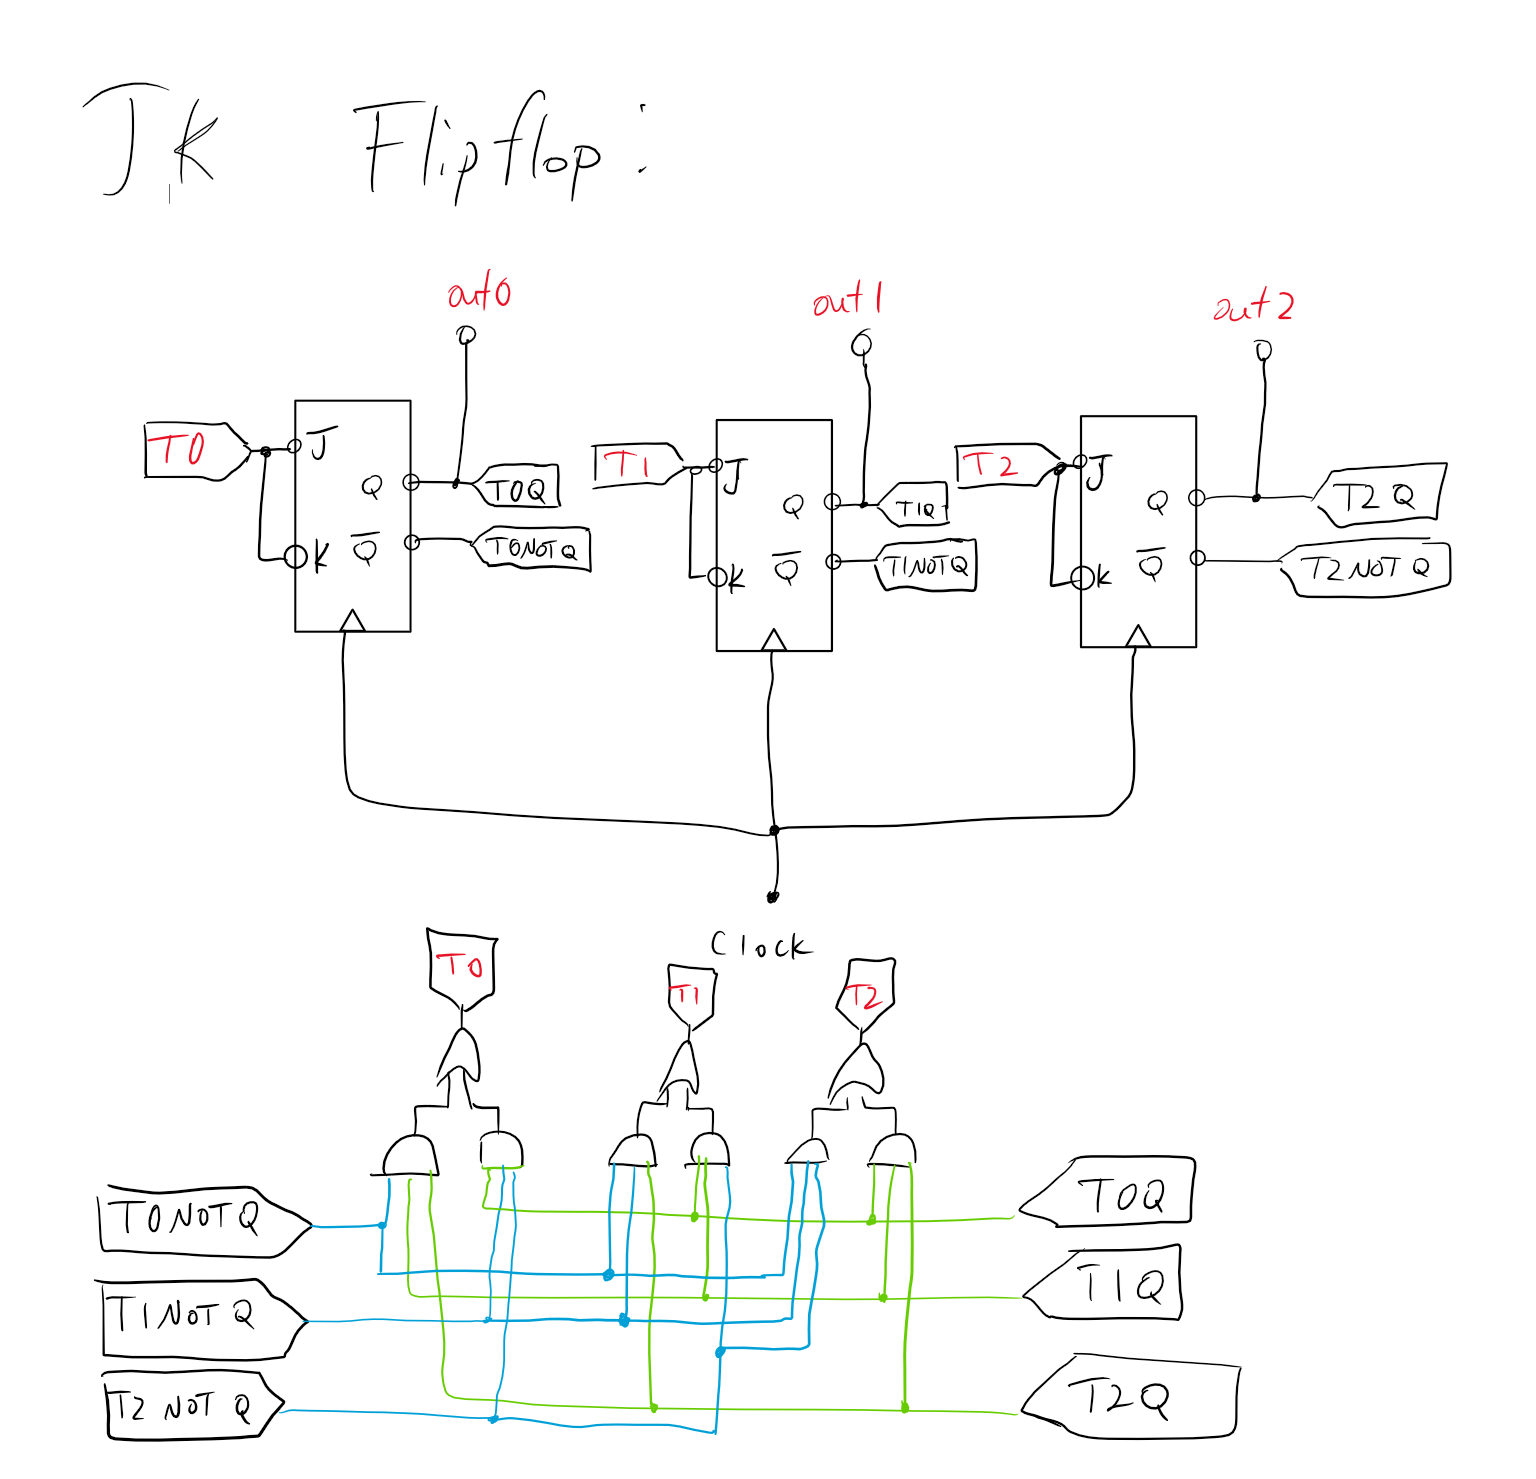
\includegraphics[scale=0.4]{jkff}
  \end{enumerate}
  \item One reason to not use latches in a 4-bit shifter is that it takes an entire cycle for a single shift. So, if I wanted to shift four bits four times, then I would have to wait at least four cycles for this action to complete, whereas, without latches, this could be done within a single cycle. For example, if you had four D Flipflops with four outputs (similar to the one below), and your goal was to set all bits to 1, then, it would take at least four cycles to reach your goal: \\ \\

  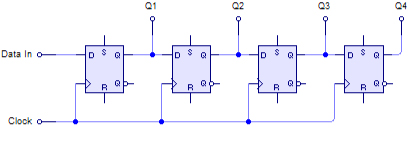
\includegraphics[scale=0.5]{wiki} \\ Source: Wikipedia (Refer to link in Homework 6 description) \\ \\
  \begin{tabular}{|l|llll|}
    \hline
    Cycle \# & \multicolumn{4}{|l|}{Q Values (q0, q1, q2, q3)} \\
    \hline
    1        & 0         & 0         & 0         & 0         \\
    2        & 1         & 0         & 0         & 0         \\
    3        & 1         & 1         & 0         & 0         \\
    4        & 1         & 1         & 1         & 0         \\
    5        & 1         & 1         & 1         & 1  \\
    \hline
  \end{tabular}
\end{enumerate}


\end{document}
